\documentclass[10pt]{article}
\usepackage[hmargin=0.8in,vmargin=0.65in]{geometry}
\usepackage{amsmath,amssymb}
\usepackage{longtable,booktabs,array}
\usepackage{graphicx}
\graphicspath{{plans/active/figures/}{figures/}}
\usepackage{algorithm}
\usepackage{algpseudocode}
\algrenewcommand\algorithmicrequire{\textbf{Input:}}
\algrenewcommand\algorithmicensure{\textbf{Output:}}
\usepackage[hidelinks]{hyperref}
% Compact spacing without shrinking equations or plot labels.
\setlength{\textfloatsep}{10pt plus 2pt minus 2pt}
\setlength{\floatsep}{8pt plus 2pt minus 2pt}
\setlength{\intextsep}{8pt plus 2pt minus 2pt}
\setlength{\abovecaptionskip}{4pt}
\setlength{\belowcaptionskip}{0pt}
\setlength{\LTpre}{4pt}
\setlength{\LTpost}{4pt}
\renewcommand{\topfraction}{0.9}
\renewcommand{\bottomfraction}{0.85}
\renewcommand{\textfraction}{0.08}
\renewcommand{\floatpagefraction}{0.8}
\setcounter{topnumber}{4}
\setcounter{bottomnumber}{3}
\setcounter{totalnumber}{6}
\makeatletter
\renewcommand\section{\@startsection{section}{1}{\z@}{-1.6ex plus -.4ex}{.7ex}{\normalfont\large\bfseries}}
\renewcommand\subsection{\@startsection{subsection}{2}{\z@}{-1.1ex plus -.3ex}{.5ex}{\normalfont\normalsize\bfseries}}
\makeatother
\AtBeginDocument{%
  \setlength{\abovedisplayskip}{6pt plus 2pt minus 2pt}%
  \setlength{\belowdisplayskip}{6pt plus 2pt minus 2pt}%
  \setlength{\abovedisplayshortskip}{3pt}%
  \setlength{\belowdisplayshortskip}{4pt}%
}
\title{Project Update:\\Multi-Agent Housing and Insurance Market}
\author{}
\date{October 28, 2026}

\begin{document}
\begin{center}
{\Large\bfseries Project Update: Multi-Agent Housing and Insurance Market\par}
\vspace{4pt}
October 28, 2026
\end{center}

\begin{abstract}
We model a housing and insurance market whose participants are RL agents with unequal incomes, property holdings, and exposure to disaster losses. We have constructed initial conditions using Lorenz curves to allocate income and ownership shares among agents, a smoothed Gaussian field to represent geographic variation in home values, and income-dependent residence assignment. Poisson event counts determine when disaster zones occur. Each zone covers neighboring homes whose modeled values fall to zero, representing total damage and displacement. These choices capture selected features of real markets under simplifying assumptions: fixed external income, concentrated ownership, and total property loss within an affected area. The environment connects these conditions to rental payments, insurance offers, coverage choices, and claims.
\end{abstract}

\section{Market model and assumptions}
RL agents represent individual market participants and insurance firms. Individual agents may be renters, owner-occupiers, or landlords according to their housing relationships. Insurer agents offer coverage to these participants. Our environment establishes the resources and risks under which they interact.

The distributions encode assumptions about real-world markets. Lorenz curves specify how income and property ownership are shared unequally among individual agents. A common ranking associates higher income with larger property portfolios. Spatially correlated prices represent expensive and inexpensive neighborhoods, while noisy residence assignment allows income and location to be related without fixing them exactly.

Disasters create geographically shared losses. We use Poisson counts to control their frequency and a fixed footprint to hold event size constant. Fixed housing supply, recurring external income, and total destruction are toy-model assumptions, not an empirical calibration. The implemented environment connects these initial conditions to rent, coverage purchases, displacement, and claim payments.

\begin{figure}[!htbp]
\centering
\setlength{\unitlength}{1pt}
\begin{picture}(430,135)
\put(5,97){\framebox(115,28){\shortstack{Person 1\\Owner-occupier}}}
\put(157,97){\framebox(115,28){\shortstack{Person 2\\Landlord}}}
\put(310,97){\framebox(115,28){\shortstack{Person 3\\Renter}}}
\put(5,5){\framebox(115,28){\shortstack{Home A\\Residence of person 1}}}
\put(255,5){\framebox(170,28){\shortstack{Home B\\Residence of person 3}}}
\put(62,97){\vector(0,-1){64}}
\put(68,57){\makebox(90,16)[l]{\small Owns and occupies}}
\put(214,97){\line(0,-1){44}}
\put(214,53){\line(1,0){77}}
\put(291,53){\vector(0,-1){20}}
\put(231,57){\makebox(45,14){\small Owns}}
\put(367,97){\vector(0,-1){64}}
\put(371,57){\makebox(55,16)[l]{\small Occupies}}
\put(310,111){\vector(-1,0){38}}
\put(270,118){\makebox(39,14){\small Rent}}
\end{picture}
\caption{Housing relationships: person 1 owns their residence; person 3 rents from person 2. Roles can overlap or change.}
\label{fig:housing-market}
\end{figure}

\section{Environment and notation}
We represent homes on an $m\times n$ grid, with $H=mn$ homes, $N$ people, and $F$ insurers. Each cell identifies one home and its location. The baseline uses $N=H$ and houses everyone, allowing us to vary inequality while holding housing availability fixed.

Matrices index homes by location; vectors index people.

\subsection{Definitions and glossary}
Let $i$ index people, $t$ simulation periods, and $(a,b)$ and $(u,v)$ home locations. Their domains are
\begin{equation}
\begin{aligned}
 m,n,N,F &\in\mathbb{Z}_{>0}, & H&=mn,\\
 i &\in\{1,\ldots,N\}, & t&\in\mathbb{Z}_{\geq0},\\
 (a,b),(u,v) &\in\{1,\ldots,m\}\times\{1,\ldots,n\}.
\end{aligned}
\end{equation}
The matrices describe homes and the vectors describe people. Quantities are current unless stated otherwise.

\renewcommand{\arraystretch}{1.08}
\begin{longtable}{@{}p{0.10\textwidth}p{0.29\textwidth}p{0.56\textwidth}@{}}
\toprule
\textbf{Symbol} & \textbf{Domain} & \textbf{Meaning} \\
\midrule
\endfirsthead
\toprule
\textbf{Symbol} & \textbf{Domain} & \textbf{Meaning (continued)} \\
\midrule
\endhead
\bottomrule
\endfoot
$P$ & $\mathbb{R}_{\geq0}^{m\times n}$ & Home values. \\
$O$ & $\{1,\ldots,N\}^{m\times n}$ & Owners, represented by person indices. \\
$R$ & $\{0,\ldots,N\}^{m\times n}$ & Residents; zero denotes vacancy. \\
$D$ & $\{0,1\}^{m\times n}$ & Destruction indicators; one denotes an uninhabitable home. \\
$\mathbf{y}$ & $\mathbb{R}_{\geq0}^{N}$ & Fixed annual external incomes. \\
$\mathbf{c}$ & $\mathbb{R}_{\geq0}^{N}$ & Cash balances. \\
\end{longtable}

Initially, $P\in\mathbb{R}_{>0}^{m\times n}$, $D=0$, and each person appears once in $R$. Ownership indices may repeat. A tenancy occurs where $R_{ab}>0$ and $R_{ab}\ne O_{ab}$. After displacement, a person may have no residence.

The ownership indicator $\mathbf{1}_{\{O_{ab}=i\}}$ identifies homes belonging to person $i$. Their home count and property wealth are
\begin{equation}
\begin{aligned}
 \text{home count of person }i &= \sum_{a=1}^{m}\sum_{b=1}^{n}\mathbf{1}_{\{O_{ab}=i\}},\\
 \text{property wealth of person }i &= \sum_{a=1}^{m}\sum_{b=1}^{n}P_{ab}\mathbf{1}_{\{O_{ab}=i\}}.
\end{aligned}
\end{equation}

\begin{figure}[!htbp]
\centering
\[
\underbrace{\begin{bmatrix}200&300\\400&500\end{bmatrix}}_{P\text{ (thousands)}}
\qquad
\underbrace{\begin{bmatrix}3&4\\3&4\end{bmatrix}}_{O\text{ (owners)}}
\qquad
\underbrace{\begin{bmatrix}1&2\\3&4\end{bmatrix}}_{R\text{ (residents)}}
\]
\caption{Illustrative allocation: people 1 and 2 rent from 3 and 4. Each owner holds two homes, worth 600 and 800 thousand respectively.}
\label{fig:matrices}
\end{figure}

Contracts link people, insurers, homes, and coverage terms. Starting capital and rents are configurable.

\subsection{Distribution functions and parameters}
\begin{longtable}{@{}p{0.10\textwidth}p{0.29\textwidth}p{0.56\textwidth}@{}}
\toprule
\textbf{Symbol} & \textbf{Domain} & \textbf{Definition} \\
\midrule
\endfirsthead
\toprule
\textbf{Symbol} & \textbf{Domain} & \textbf{Definition (continued)} \\
\midrule
\endhead
\bottomrule
\endfoot
$L_y,L_h$ & $[0,1]\to[0,1]$ & Lorenz functions for income and home counts along the same person ordering. \\
$\mu$ & $\mathbb{R}_{>0}$ & Mean annual external income. \\
$\Delta t$ & $\mathbb{R}_{>0}$ & Period length in years. \\
$p_0$ & $\mathbb{R}_{>0}$ & Reference home price. \\
$\sigma,\ell$ & $\mathbb{R}_{\geq0}$ & Log-price variation and spatial smoothing scale. \\
$\tau$ & $\mathbb{R}_{\geq0}$ & Noise strength for residence placement. \\
$\lambda_t$ & $\mathbb{R}_{\geq0}$ & Expected disasters in period $t$. \\
$S$ & $\mathbb{Z}_{\geq0}$ & Global seed for labeled component random streams. \\
\end{longtable}

People are indexed by nondecreasing income, with seeded tie-breaking. Auxiliary quantities are defined below.

\section{Assigning initial home values}
We introduce spatial price variation so agents face properties with different values and geographic concentrations of potential loss. Let $E\in\mathbb{R}^{m\times n}$ be the seeded noise matrix, with one independent draw per home:
\begin{equation}
 E_{ab}\overset{\mathrm{iid}}{\sim}\mathcal{N}(0,1).
\end{equation}
For a smoothing scale $\ell>0$, let $w_{ab,uv}$ be the weight of cell $(u,v)$ when constructing the field at $(a,b)$. Define the smoothing operator $\mathcal{S}_{\ell}$ using these distance-based weights:
\begin{equation}
\begin{aligned}
 w_{ab,uv}
 &=\exp\left(-\dfrac{(a-u)^2+(b-v)^2}{2\ell^2}\right),\\[8pt]
 [\mathcal{S}_{\ell}(E)]_{ab}
 &=\dfrac{\displaystyle\sum_{u=1}^{m}\sum_{v=1}^{n}w_{ab,uv}E_{uv}}
 {\displaystyle\sqrt{\sum_{u=1}^{m}\sum_{v=1}^{n}w_{ab,uv}^{2}}}.
\end{aligned}
\end{equation}
The scale $\ell$ controls neighborhood size; normalization gives unit variance at each cell. Boundaries do not wrap. With no smoothing, define $\mathcal{S}_0(E)=E$.

Using reference price $p_0$ and log-price spread $\sigma$, the initial price matrix is
\begin{equation}
 P=p_0\exp\left(\sigma\mathcal{S}_{\ell}(E)\right).
\end{equation}
The exponential acts entrywise, giving positive prices with median $p_0$ at each cell. Prices are generated independently of population allocation. The baseline rounds values to cents and uses pre-loss market value for building claims.

\begin{figure}[!htbp]
\centering
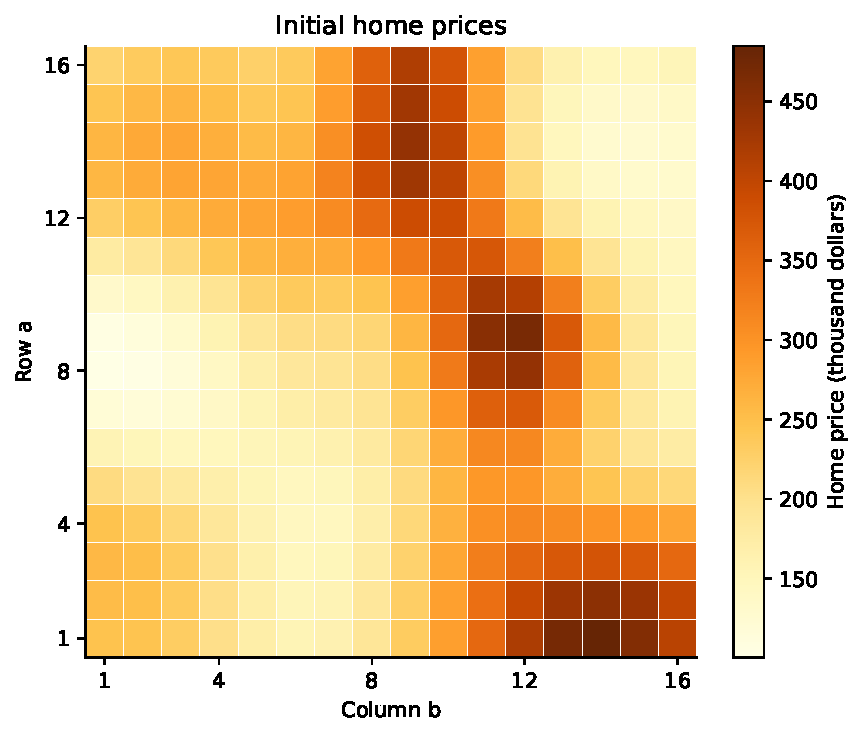
\includegraphics[width=0.48\textwidth]{initial-prices.pdf}
\caption{Each cell is one home; color shows its initial price generated from seeded spatial noise. Example: $m=n=16$, $S=42$, $p_0=250{,}000$, $\sigma=0.4$, $\ell=2$.}
\label{fig:price-distribution}
\end{figure}

\begin{algorithm}[H]
\caption{Generate initial home values}
\label{alg:prices}
\begin{algorithmic}[1]
\Require Grid dimensions, $p_0,\sigma,\ell$, and seeded price stream
\State Draw $E_{ab}\overset{\mathrm{iid}}{\sim}\mathcal{N}(0,1)$
\State $P\gets p_0\exp\bigl(\sigma\mathcal{S}_{\ell}(E)\bigr)$; $D\gets0$
\State \Return $P,D$
\end{algorithmic}
\end{algorithm}

\section{Assigning income and ownership shares}
Lorenz curves model inequality by specifying cumulative income and ownership shares among individual RL agents. Separate curves allow different concentrations of income and home counts; the shared income ranking associates higher earnings with larger intended portfolios. Their totals are $N\mu$ dollars per year and $H$ homes.

For either Lorenz curve $L\in\{L_y,L_h\}$, let $\mathbf{d}(L)\in[0,1]^N$ contain the individual shares. Person $i$ receives the increase in cumulative share over their population interval:
\begin{equation}
 [\mathbf{d}(L)]_i
 =L\left(\dfrac{i}{N}\right)
 -L\left(\dfrac{i-1}{N}\right),
 \qquad i\in\{1,\ldots,N\}.
\end{equation}
Let $y_i$ be person $i$'s annual income and $a_i$ their fractional target number of homes. Multiplying the corresponding shares by total income and housing supply gives
\begin{equation}
\begin{aligned}
 y_i&=N\mu\left[
 L_y\left(\dfrac{i}{N}\right)-L_y\left(\dfrac{i-1}{N}\right)
 \right],\\[3pt]
 a_i&=H\left[
 L_h\left(\dfrac{i}{N}\right)-L_h\left(\dfrac{i-1}{N}\right)
 \right].
\end{aligned}
\end{equation}
Let $\mathbf{a}\in\mathbb{R}_{\geq0}^{N}$ collect the fractional targets and $\mathbf{h}\in\mathbb{Z}_{\geq0}^{N}$ the whole-home allocations. Obtain $\mathbf{h}$ by rounding and correcting the total:
\begin{enumerate}
\item Round each $a_i$ to the nearest integer, rounding halves upward.
\item If $\sum_i h_i<H$, add one to the count with largest $a_i-h_i$.
\item If $\sum_i h_i>H$, subtract one from a positive count with largest $h_i-a_i$.
\end{enumerate}
Repeat the applicable correction until the total is $H$, recomputing differences and breaking ties by seed. The curve targets counts; property wealth follows from the assigned homes.

Income remains fixed after initialization. Its contribution to cash over one period is
\begin{equation}
 \mathbf{c}\gets\mathbf{c}+\Delta t\,\mathbf{y}.
\end{equation}
The baseline configures starting cash and rent separately. Each period credits income before rent, disasters, and claims.

\begin{figure}[!htbp]
\centering
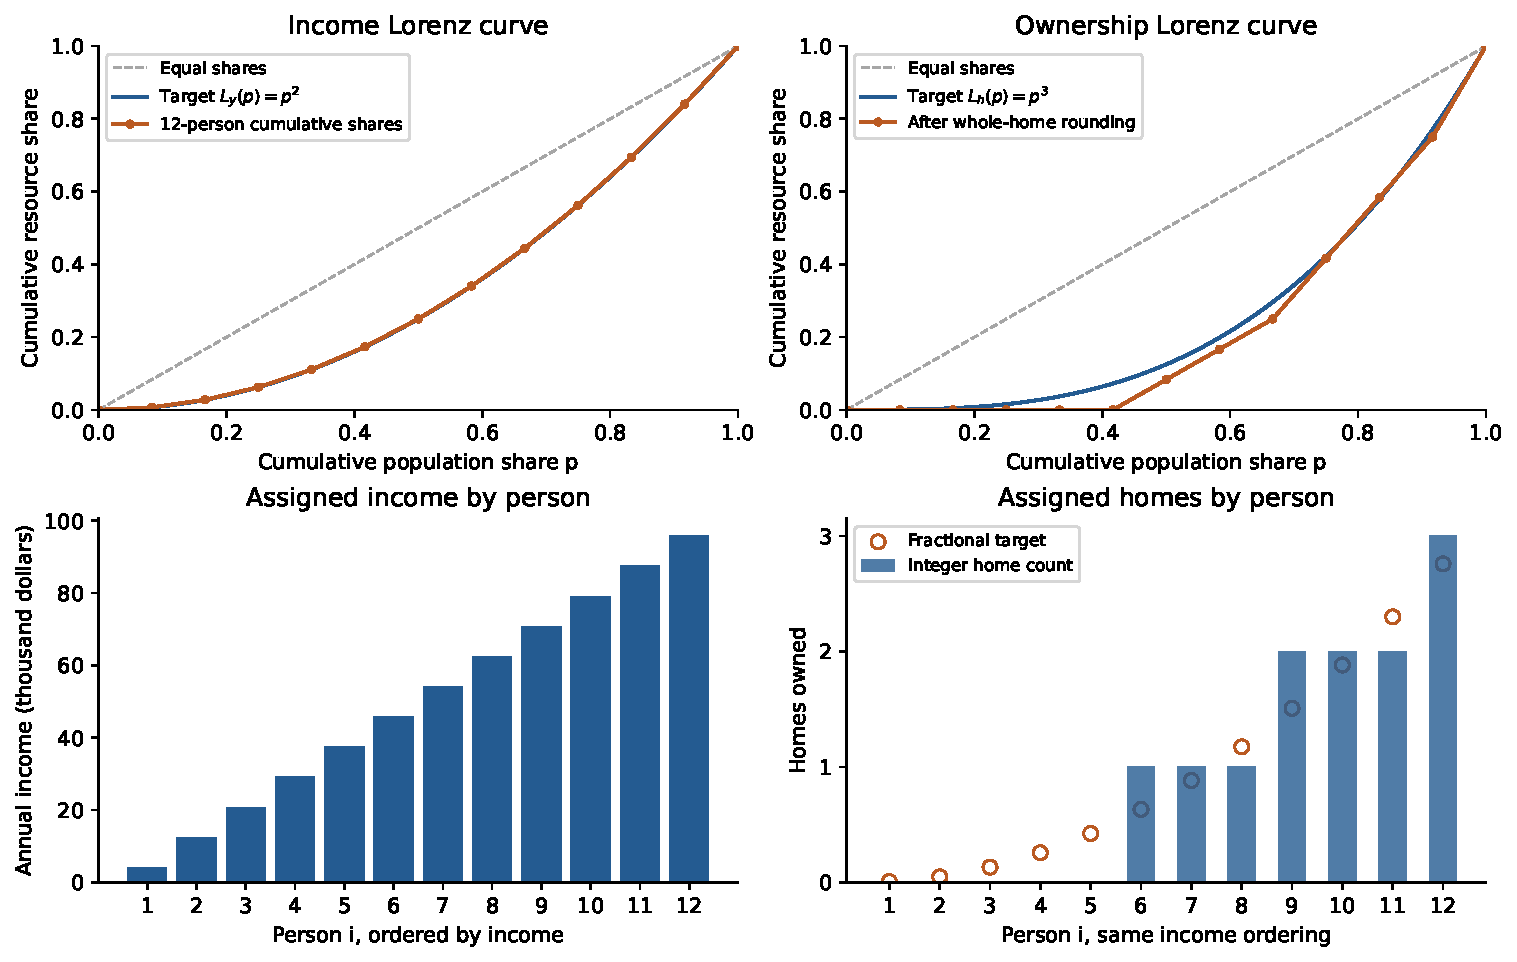
\includegraphics[width=0.88\textwidth]{lorenz-allocations.pdf}
\caption{Illustrative allocation: $N=H=12$, $\mu=50{,}000$, $L_y(p)=p^2$, $L_h(p)=p^3$. Markers show finite-population shares; lower panels show incomes and integer home counts against fractional targets. These settings are not empirical calibration.}
\label{fig:lorenz-distributions}
\end{figure}

\begin{algorithm}[H]
\caption{Assign incomes and home counts}
\label{alg:incomes}
\begin{algorithmic}[1]
\Require $N,H,\mu,L_y,L_h$ and seeded tie-breaking
\State $\mathbf{y}\gets N\mu\mathbf{d}(L_y)$; $\mathbf{a}\gets H\mathbf{d}(L_h)$
\State Round each $a_i$ to the nearest integer $h_i$, with halves rounded upward
\State Correct largest rounding residuals until $\sum_i h_i=H$, as specified above
\State \Return $\mathbf{y},\mathbf{h}$
\end{algorithmic}
\end{algorithm}

\section{Connecting people to homes}
Residence and ownership determine who pays rent, receives it, or loses housing in a disaster. We assign residences with an income bias while retaining random variation.

For person $i$, let $B_i$ contain people with lower income and $T_i$ contain people with the same income:
\[
\begin{aligned}
 B_i &:= \{j\in\{1,\ldots,N\}:y_j<y_i\},
 & &\text{lower-income people},\\[5pt]
 T_i &:= \{j\in\{1,\ldots,N\}:y_j=y_i\},
 & &\text{equal-income people}.
\end{aligned}
\]
Let $r_i\in[0,1]$ be the income percentile, $z_i\in\mathbb{R}$ an independent noise draw, and $q_i\in\mathbb{R}$ the placement score. Using $|B_i|$ and $|T_i|$ for the respective group sizes, define
\begin{equation}
\begin{aligned}
 r_i &:= \dfrac{|B_i|+\dfrac{1}{2}|T_i|}{N},
 & &\text{income percentile},\\[8pt]
 z_i &\overset{\mathrm{iid}}{\sim}\mathcal{N}(0,1),
 & &\text{placement noise},\\[5pt]
 q_i &:= r_i+\tau z_i,
 & &\text{placement score}.
\end{aligned}
\end{equation}
Match people ranked by $\mathbf{q}$ to homes ranked by price. Equal incomes receive equal percentiles; ties are broken by seed. Increasing $\tau$ weakens income-based sorting. An independent baseline uses random assignment.

Second, we assign titles using the quotas from the original income ranking. Each positive-quota owner receives their residence first, then additional homes up to their quota. Nonowners become renters. With $H=N$, residual ownership capacity exactly covers their residences. This assignment does not enforce affordability; initial rent is configured separately.

Remaining titles are assigned by shuffling owner-capacity slots. This samples slots uniformly, so owners with larger remaining quotas receive proportionally more opportunities.

\begin{algorithm}[H]
\caption{Assign residences and ownership}
\label{alg:board}
\begin{algorithmic}[1]
\Require $P,\mathbf{y},\mathbf{h},\tau$ and seeded placement and ownership streams
\State Compute income percentiles $\mathbf{r}$ and draw $z_i\overset{\mathrm{iid}}{\sim}\mathcal{N}(0,1)$
\State Match people ranked by $q_i=r_i+\tau z_i$ to cells ranked by price, filling $R$
\State Give each person with $h_i>0$ ownership of their residence
\State Shuffle residual owner-capacity slots and assign remaining titles, filling $O$
\State \Return $R,O$
\end{algorithmic}
\end{algorithm}

One global seed supplies independent streams for generation, placement, ownership, and disasters.

\section{Introducing insurance choices}
Each insurer can offer homeowners, landlord, and renters coverage. The implemented opening round collects firm offers and person choices before disaster exposure. Premiums are paid up front for fixed-term contracts. The example uses fixed quotes and cheapest-affordable purchasing; learned pricing and purchasing policies will replace these baselines.

For a covered loss, payment due is the loss minus the deductible, bounded below by zero and above by the coverage limit. Actual payment is capped by available insurer capital, with any shortfall recorded. Building losses use pre-disaster home values; renters' contents losses use an explicit contract amount. These are provisional toy settlement rules.

\begin{figure}[!htbp]
\centering
\setlength{\unitlength}{1pt}
\begin{picture}(430,155)
\put(5,120){\framebox(125,28){\shortstack{Owner-occupier\\Homeowners coverage}}}
\put(152,120){\framebox(125,28){\shortstack{Landlord\\Landlord coverage}}}
\put(299,120){\framebox(125,28){\shortstack{Renter\\Renters coverage}}}
\put(67,120){\line(0,-1){15}}
\put(214,120){\line(0,-1){15}}
\put(361,120){\line(0,-1){15}}
\put(67,105){\line(1,0){294}}
\put(130,105){\vector(0,-1){57}}
\put(35,70){\makebox(85,18){\small Premiums}}
\put(330,48){\vector(0,1){57}}
\put(163,65){\makebox(155,30){\shortstack{\small Offers and covered\\\small claim payments}}}
\put(5,0){\framebox(419,48){}}
\put(10,30){\makebox(409,15){\small Competing insurer RL agents}}
\put(20,6){\framebox(115,20){Firm A}}
\put(157,6){\framebox(115,20){Firm B}}
\put(294,6){\framebox(115,20){Firm C}}
\end{picture}
\caption{Housing roles determine applicable coverage. People choose among competing firms; arrows represent market access and contractual payments.}
\label{fig:insurance-market}
\end{figure}

An owner and tenant may insure different losses at the same home with different firms. One disaster can therefore affect several agents and contracts.

\begin{algorithm}[H]
\caption{Open the insurance market}
\label{alg:insurance}
\begin{algorithmic}[1]
\Require Housing allocation, cash, insurer capital, and decision policies
\State Collect all insurer offers, then each person's coverage choices
\State Validate eligibility and affordability; transfer accepted premiums
\State Activate contracts and return updated balances
\end{algorithmic}
\end{algorithm}

\section{Introducing disaster exposure}
A disaster creates a damage zone on the housing grid. Homes inside that zone become uninhabitable and their modeled values fall to zero; homes outside it retain their values for that event. This represents a local shock affecting several neighboring properties rather than unrelated losses scattered across the market.

We separate the occurrence of a disaster from its spatial extent. Poisson counts determine the number of events in a period. Each event then receives a randomly located zone of fixed size, so changing the rate changes frequency without changing the area damaged by each event. Let $K_t\in\mathbb{Z}_{\geq0}$ count disasters in period $t$, with expected count $\lambda_t$. Let $f(k;\lambda_t)$ denote the probability of $k$ events. Period counts are independent conditional on the rate schedule:
\begin{equation}
\begin{aligned}
 K_t&\sim\operatorname{Poisson}(\lambda_t),\\[3pt]
 f(k;\lambda_t)
 &=\Pr(K_t=k)
 =\dfrac{\lambda_t^k e^{-\lambda_t}}{k!},
 \qquad k\in\mathbb{Z}_{\geq0}.
\end{aligned}
\end{equation}
At $\lambda_t=0$, $\Pr(K_t=0)=1$. The baseline uniformly samples eligible positions for a fixed rectangle fully contained in the grid. Footprint size therefore remains constant at the boundary.

For an event index $e\in\{1,\ldots,K_t\}$, let $\mathcal{F}_e\subseteq\{1,\ldots,m\}\times\{1,\ldots,n\}$ contain the cells affected by event $e$. For every $(a,b)\in\mathcal{F}_e$ with $D_{ab}=0$, retain the pre-loss information and set
\begin{equation}
\begin{aligned}
 P_{ab}&\gets0,\\[4pt]
 R_{ab}&\gets0,\\[4pt]
 D_{ab}&\gets1.
\end{aligned}
\end{equation}
Zero value is our proxy for total property damage, not a price chosen by an agent. The owner retains title but loses the modeled property value; the resident loses usable housing and is displaced. These may be different agents. A landlord can therefore lose several properties in one zone while several tenants lose their residences.

Pre-disaster values and occupancy identify the losses associated with each contract. Insurers covering homes in the same zone can face multiple claims from one event. This connects the spatial setup to the concentration of insurance risk.

Overlapping zones do not generate another building loss for an already destroyed home. The total-loss rule simplifies damage severity and omits surviving land value; zero-valued homes remain uninhabitable until a recovery mechanism is introduced.

\begin{figure}[!htbp]
\centering
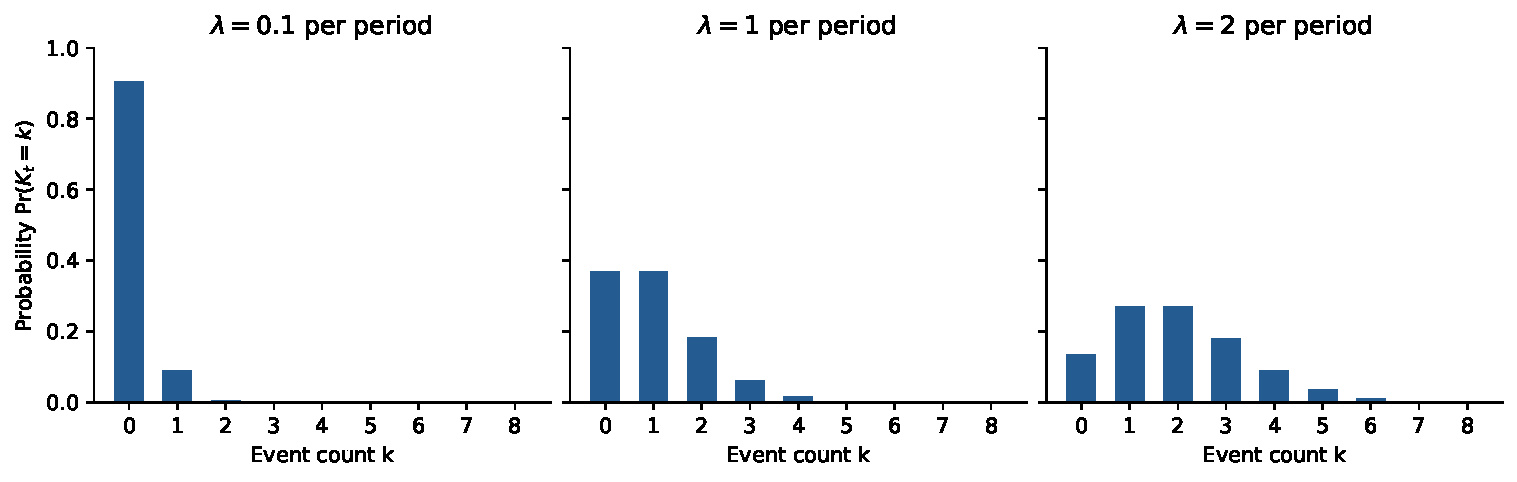
\includegraphics[width=\textwidth]{poisson-counts.pdf}
\caption{Disaster counts per period for illustrative rates, not selected simulation parameters. Displayed probability masses cover $k\in\{0,\ldots,8\}$; the omitted tail is below $0.00024$ in each panel.}
\label{fig:poisson-distribution}
\end{figure}

\begin{algorithm}[H]
\caption{Apply disasters and claims}
\label{alg:disaster}
\begin{algorithmic}[1]
\Require $P,O,R,D$, contracts, $\lambda_t$, fixed footprint, and disaster stream
\State Draw $K_t\sim\operatorname{Poisson}(\lambda_t)$
\For{$e\in\{1,\ldots,K_t\}$}
    \State Sample footprint $\mathcal{F}_e$; retain pre-loss records where $D_{ab}=0$
    \State For those cells: $P_{ab}\gets0$, $R_{ab}\gets0$, $D_{ab}\gets1$
    \State Record displaced residents and settle covered claims; retain ownership
\EndFor
\end{algorithmic}
\end{algorithm}

The baseline pays claims after each event. Replacement housing and rebuilding remain future extensions.

\section{Environment Variants}
\label{sec:environment-variants}
We propose three worlds---Peace, Standard, and Chaos---as the main experimental comparisons. They vary the initial distribution of resources and the disaster-rate schedule under which RL agents make housing and insurance decisions. Distribution parameters control inequality and spatial variation; the rate schedule controls how risk changes during an episode. In each world, agents choose actions to maximize their expected discounted cumulative rewards.

\subsection{Shared experimental controls}
Fix the population $N$, insurer count $F$, housing supply $H=N$, episode length $T\in\mathbb{Z}_{>0}$, and period duration $\Delta t$. There are $N+F$ RL agents. Let $M_0\in\mathbb{R}_{\geq0}$ be the total initial cash across people and insurers, and let $b_f(0)$ denote insurer $f$'s initial capital. Let $Y\in\mathbb{R}_{>0}$ be the population's total annual external income. These budgets satisfy
\begin{equation}
\begin{aligned}
 M_0 &= \sum_{i=1}^{N}c_i(0)+\sum_{f=1}^{F}b_f(0),
 & &\text{initial cash budget},\\[5pt]
 Y &= \sum_{i=1}^{N}y_i=N\mu,
 & &\text{annual income budget}.
\end{aligned}
\end{equation}
Initial cash and annual income are separate controls. Recurring external income adds cash during the simulation, so fixing $M_0$ does not conserve the money supply. We use $Y$ as the toy economy's income measure; a full GDP accounting model is not assumed.

Across matched runs, hold these totals, insurer starting capital, disaster footprint, insurance rules, and learning configuration fixed. Use the same set of seeds for each world. This separates differences in resource allocation and risk from differences in population or aggregate resources.

\subsection{Peace: equal initial resources}
Peace starts every person with the same income, one home, and the same cash balance. Every home has the same initial price. Let $M_{\mathrm{people}}:=M_0-\sum_{f=1}^{F}b_f(0)$ be the nonnegative cash budget assigned to people. For population share $p\in[0,1]$, choose
\begin{equation}
\begin{aligned}
 L_y(p)=L_h(p)&=p,
 & &\text{equal resource shares},\\[5pt]
 y_i&=\dfrac{Y}{N},\qquad h_i=1,
 & &\text{income and home allocation},\\[5pt]
 c_i(0)&=\dfrac{M_{\mathrm{people}}}{N},
 & &\text{equal initial cash},\\[5pt]
 P_{ab}(0)&=p_0,\qquad \sigma=0,
 & &\text{equal home values}.
\end{aligned}
\end{equation}
Each person owns their residence, so there are no initial tenancies. Income-based placement has no effect when incomes and prices are equal. Equality describes the initial state; subsequent decisions and localized losses may separate agents' outcomes.

Equal cash balances and equal-valued home holdings give every person the same initial wealth. These are initialization conditions: there is no ongoing wealth cap or redistribution rule. Agents can accumulate different incomes from property, cash balances, and holdings through subsequent interactions, while their assigned external incomes remain fixed.

For the initial comparison, Peace uses the same constant disaster rate as Standard, holding the risk schedule fixed while varying the initial resource distribution.

\subsection{Standard: unequal resources and constant risk}
Standard uses the income and ownership Lorenz curves, spatial price field, and residence assignment defined above. The tunable parameters are $L_y,L_h$, price spread $\sigma$, smoothing scale $\ell$, and placement noise $\tau$. Normalize allocations to the shared income and home totals. Hold initial personal cash equal as in Peace unless cash inequality is itself the subject of a separate experiment.

Let $\bar{\lambda}\in\mathbb{R}_{>0}$ be the selected constant expected event count per period. The reference risk schedule is
\begin{equation}
 \lambda_t=\bar{\lambda},\qquad t\in\{0,\ldots,T-1\}.
\end{equation}
Select $\bar{\lambda}$ together with episode length and footprint size; a rate is meaningful relative to how many homes each event can destroy. No numerical rate is fixed here.

\subsection{Chaos: exponentially increasing risk}
Chaos begins with the same resource allocation and insurance conditions as a matched Standard run. Only the disaster-rate schedule changes. Let $\lambda_0\in\mathbb{R}_{>0}$ be the low initial expected event count and $g\in\mathbb{R}_{>0}$ the growth parameter per simulation step. Set
\begin{equation}
\begin{aligned}
 \lambda_t&=\lambda_0\exp(gt),
 & &t\in\{0,\ldots,T-1\},\\[5pt]
 K_t&\sim\operatorname{Poisson}(\lambda_t),
 & &\text{events in period }t.
\end{aligned}
\end{equation}
The rate grows by the same factor $\exp(g)$ each step. Its absolute increase is small at first and larger later, producing an escalating period of disruption. This is exponential growth of the Poisson rate, not an exponential distribution for event counts. Events remain random, so the realized count need not increase every period.

To tune the onset, choose a target rate $\lambda_{\star}>\lambda_0$ at a step $t_{\star}\in\{1,\ldots,T-1\}$, for $T\geq2$. The required growth parameter is
\begin{equation}
 g=\dfrac{\log(\lambda_{\star}/\lambda_0)}{t_{\star}}.
\end{equation}
The footprint stays fixed. Increasing frequency therefore changes exposure without changing event severity. Since destroyed homes cannot incur another building loss and rebuilding is absent, late events may strike already damaged cells. Track newly destroyed homes and displacement alongside event counts.

\subsection{Research comparisons}
Peace versus Standard compares equal and unequal initial resource distributions under constant risk. Standard versus Chaos compares stationary with increasing risk under the same initial allocation. For a timing-only comparison, set Standard's constant rate to Chaos's mean rate over the episode:
\begin{equation}
 \bar{\lambda}=\dfrac{1}{T}\sum_{t=0}^{T-1}\lambda_0\exp(gt).
\end{equation}
This matches the expected total number of events while changing their timing. Compare RL agents' coverage choices, housing holdings, wealth concentration, displacement, and insurer solvency across repeated seeds. The three worlds are experimental configurations; changes to individual parameters provide the corresponding ablations.

\section{RL agent formulation}
\label{sec:rl-agents}
% Reserved for the RL formulation: observations, actions, rewards, and learning setup.
% This section is intentionally left for the agent write-up; it does not indicate
% the status of work undertaken outside this document.

\section{Questions for evaluation}
How do income and ownership inequality affect agents' housing and coverage decisions? How does geographic exposure influence insurer pricing and losses? Comparisons across initial distributions and disaster rates will examine these interactions under the stated assumptions.

\end{document}
